%=====================================================================
\section{Methods}\label{sec:methods}
%=====================================================================

\begin{figure}[!htbp]
\centering
\IfFileExists{figures/fig_method_hybrid.pdf}{\includegraphics[width=\textwidth]{figures/fig_method_hybrid.pdf}}{\IfFileExists{figures/fig_method_hybrid.png}{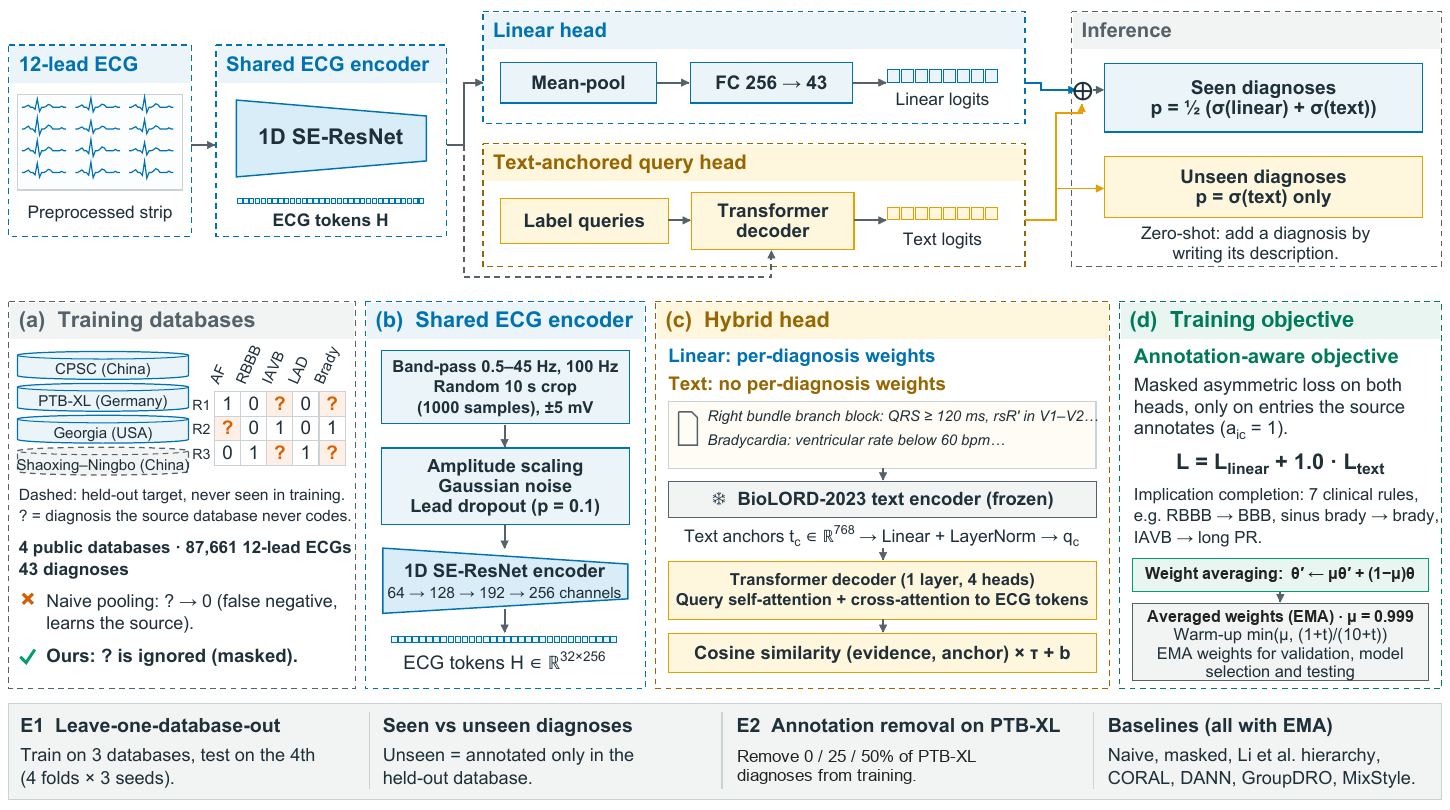
\includegraphics[width=\textwidth]{figures/fig_method_hybrid.png}}{\fbox{\parbox{0.9\textwidth}{\centering\vspace{2cm}Methodology figure (figures/fig\_method\_hybrid.pdf)\vspace{2cm}}}}}
\caption{Overview of the approach. (a) Training databases annotate different diagnosis vocabularies; an entry that a database never codes (``?'') is unknown, not negative, and naive pooling treats it as a negative. (b) A one-dimensional SE-ResNet encodes a 10\,s, 100\,Hz 12-lead recording into $T=32$ tokens. (c) Two heads read the same tokens: a linear head with one weight vector per diagnosis, and a text-anchored label-query head in which frozen clinical description embeddings (BioLORD-2023) act as queries that cross-attend to the tokens and are scored by cosine similarity, so that it has no diagnosis-specific weights. Diagnoses supervised in training are scored by the mean of the two probabilities; diagnoses never supervised are scored by the text head alone. (d) Both heads are trained with the same asymmetric loss restricted to source-annotated entries, after completion of positives through seven clinical implication rules; an exponential moving average of the weights is validated, selected and tested. The bottom strip lists the evaluation protocols.}\label{fig:method}
\end{figure}

\subsection{Overview}\label{sec:overview}
The method has four components, summarized in Table~\ref{tab:components}, each tied to one aspect of the problem. A one-dimensional residual encoder maps a 12-lead recording to a short sequence of tokens (Section~\ref{sec:encoder}). A \emph{hybrid head} reads these tokens twice (Section~\ref{sec:head}): a conventional linear head provides the discriminative capacity of per-diagnosis weights on diagnoses that the training sources annotate, and a text-anchored label-query head scores every diagnosis from a frozen embedding of its clinical description, so that diagnoses without any training label remain scorable (RQ3). An annotation-aware objective restricts the loss of both heads to entries that the record's source annotates and completes positives through implication rules (RQ1, Section~\ref{sec:objective}). Finally, model selection and inference use an exponential moving average of the weights, which stabilizes the selected model across the distribution shift between validation sources and the held-out database (RQ2, Section~\ref{sec:train}). Section~\ref{sec:why} formalizes why the naive pooled objective is misspecified and motivates the masked objective. Notation is summarized in Table~\ref{tab:notation}. The design was arrived at through a development process with selection rules fixed in advance; it is reported, with its negative intermediate results and one deviation from those rules, in Appendix~\ref{secA2}.

\begin{table}[!htbp]
\centering\footnotesize
\caption{Components of the method, the problem each addresses and where it is defined.}\label{tab:components}
\begin{tabularx}{\textwidth}{@{}l X X l@{}}
\toprule
Component & Problem addressed & Mechanism & Defined in \\
\midrule
ECG encoder & Variable-length, multi-rate recordings & Band-pass, 100\,Hz, random 10\,s crops; SE-ResNet tokens & Sec.~\ref{sec:encoder} \\
Linear head & Discriminative power on annotated diagnoses & Mean-pooled tokens, one weight vector per diagnosis & Eq.~\eqref{eq:linear} \\
Text-anchored head & Fixed label set; unseen diagnoses not scorable & Frozen description embeddings as queries; cosine scoring & Eqs.~\eqref{eq:query}--\eqref{eq:logit} \\
Score fusion & Combining both heads without losing open vocabulary & Mean probability on seen diagnoses, text head on unseen ones & Eq.~\eqref{eq:fusion} \\
Masked asymmetric loss & Unannotated entries treated as negatives & Loss on both heads, only on source-annotated entries & Eqs.~\eqref{eq:lann}--\eqref{eq:total} \\
Implication completion & Coarse findings implied but not coded & Seven child\,$\rightarrow$\,parent rules on targets & Eq.~\eqref{eq:rules} \\
Weight averaging & Unstable selection under source shift & EMA of weights with warm-up; EMA validated and tested & Eq.~\eqref{eq:ema} \\
\bottomrule
\end{tabularx}
\end{table}

\subsection{Problem formulation}\label{sec:problem}
Let $\mathcal{S}=\{1,\dots,S\}$ index the source databases and let $\mathcal{V}=\{1,\dots,C\}$ be a global diagnosis vocabulary. Source $s$ annotates a subset $\mathcal{V}_s\subseteq\mathcal{V}$; we define $\mathcal{V}_s$ operationally as the diagnoses with at least ten positive recordings in $s$ (Section~\ref{sec:data}). A training record is a tuple $(\mathbf{x}_i, \mathbf{y}_i, \mathbf{a}_i, s_i)$, where $\mathbf{x}_i\in\mathbb{R}^{12\times L}$ is a 12-lead ECG, $y_{ic}\in\{0,1\}$ indicates that diagnosis $c$ was coded, and $a_{ic}=\mathbbm{1}[c\in\mathcal{V}_{s_i}]$ indicates that $y_{ic}$ is \emph{observed}. When $a_{ic}=0$ the value $y_{ic}=0$ means ``not annotated'' rather than ``absent''. The goal is a scorer $p_c(\mathbf{x})\in[0,1]$ that performs well on a target database $s^\ast\notin\mathcal{S}$, both on the diagnoses that some training source annotates, $\mathcal{V}_{\mathrm{seen}}=\bigcup_{s\in\mathcal{S}}\mathcal{V}_s$, and on the diagnoses $\mathcal{V}_{s^\ast}\setminus\mathcal{V}_{\mathrm{seen}}$ that only the target annotates. We write $\kappa_c=\mathbbm{1}[c\in\mathcal{V}_{\mathrm{seen}}]$.

\begin{table}[!htbp]
\centering\footnotesize
\caption{Notation.}\label{tab:notation}
\begin{tabularx}{\textwidth}{@{}l X@{}}
\toprule
Symbol & Meaning \\
\midrule
$\mathcal{S}$, $S$ & Set and number of training source databases; $s^\ast$ is the held-out target database \\
$\mathcal{V}$, $C$ & Global diagnosis vocabulary and its size; $\mathcal{V}_s\subseteq\mathcal{V}$ the diagnoses annotated by source $s$ \\
$\mathbf{x}_i\in\mathbb{R}^{12\times L}$ & 12-lead recording $i$ at 100\,Hz; $L=1000$ for a 10\,s training crop \\
$y_{ic}\in\{0,1\}$ & Diagnosis $c$ coded for record $i$ \\
$a_{ic}\in\{0,1\}$ & Entry $(i,c)$ observed, i.e.\ $c\in\mathcal{V}_{s_i}$ \\
$\kappa_c\in\{0,1\}$ & Diagnosis $c$ annotated by at least one training source (seen) \\
$\mathbf{H}\in\mathbb{R}^{T\times D}$ & ECG token sequence from the encoder $f_\theta$; $T=32$, $D=256$ \\
$\bar{\mathbf{h}}\in\mathbb{R}^{D}$ & Mean of the $T$ tokens \\
$\mathbf{t}_c\in\mathbb{R}^{768}$ & Frozen text embedding (anchor) of the description of diagnosis $c$ \\
$\mathbf{q}_c\in\mathbb{R}^{D}$ & Label-specific evidence vector for diagnosis $c$ after the decoder \\
$\ell^{\mathrm{lin}}_c$, $\ell^{\mathrm{txt}}_c$ & Logits of diagnosis $c$ from the linear and the text-anchored head \\
$p_c$ & Reported probability for diagnosis $c$ (Eq.~\eqref{eq:fusion}) \\
$\tau$, $b$ & Learned scalar scale and bias of the text head \\
$\phi(\ell,y)$ & Asymmetric loss for one entry, as a function of the logit \\
$\theta$, $\bar\theta$ & Trained parameters and their exponential moving average; $\mu$ the EMA momentum \\
$\lambda_{\mathrm{txt}}$ & Weight of the text-head loss \\
$\mathcal{R}$ & Set of clinical implication rules $(c\rightarrow c')$ \\
$B$ & Mini-batch size \\
\bottomrule
\end{tabularx}
\end{table}

\subsection{Why naive pooling fails}\label{sec:why}
Naive pooling concatenates the databases and trains on the target $\tilde y_{ic}=y_{ic}a_{ic}$, so that every unannotated entry becomes a zero. The following proposition, a direct consequence of the well-known fact that cross-entropy is minimized by the conditional expectation of the target, makes explicit what such a model estimates. We state it for one diagnosis $c$ and drop the index.

\begin{proposition}\label{prop:naive}
Let $(\mathbf{x},y,a)$ be jointly distributed with $y,a\in\{0,1\}$, and let the model class be rich enough that the expected binary cross-entropy $\mathbb{E}[-\tilde y\log p(\mathbf{x})-(1-\tilde y)\log(1-p(\mathbf{x}))]$ can be minimized pointwise in $\mathbf{x}$. Then the naive minimizer is $p^\ast_{\mathrm{naive}}(\mathbf{x})=P(y=1,a=1\mid\mathbf{x})$, and the minimizer of the masked objective $\mathbb{E}[a\,(-y\log p(\mathbf{x})-(1-y)\log(1-p(\mathbf{x})))]$ is $p^\ast_{\mathrm{mask}}(\mathbf{x})=P(y=1\mid\mathbf{x},a=1)$ wherever $P(a=1\mid\mathbf{x})>0$. If, in addition, $y$ and $a$ are conditionally independent given $\mathbf{x}$, then
\begin{equation}
p^\ast_{\mathrm{naive}}(\mathbf{x})=P(y=1\mid\mathbf{x})\,P(a=1\mid\mathbf{x}),
\qquad
p^\ast_{\mathrm{mask}}(\mathbf{x})=P(y=1\mid\mathbf{x}).
\label{eq:prop}
\end{equation}
\end{proposition}

\begin{proof}
For a fixed $\mathbf{x}$ the naive risk is $-\eta\log p-(1-\eta)\log(1-p)$ with $\eta=\mathbb{E}[\tilde y\mid\mathbf{x}]=P(y=1,a=1\mid\mathbf{x})$, since $\tilde y=ya$ is a product of indicators; this function of $p\in(0,1)$ is minimized at $p=\eta$. For the masked risk, conditioning on $\mathbf{x}$ gives $P(a=1\mid\mathbf{x})\,[-\eta'\log p-(1-\eta')\log(1-p)]$ with $\eta'=\mathbb{E}[y\mid\mathbf{x},a=1]$, minimized at $p=\eta'$ whenever the prefactor is positive. Conditional independence factorizes $P(y=1,a=1\mid\mathbf{x})=P(y=1\mid\mathbf{x})P(a=1\mid\mathbf{x})$ and gives $P(y=1\mid\mathbf{x},a=1)=P(y=1\mid\mathbf{x})$.
\end{proof}

Two consequences follow. First, naive predictions are deflated by $P(a=1\mid\mathbf{x})$, the probability that the recording comes from a source that annotates $c$; a diagnosis coded by one of three sources is systematically under-scored. Second, and more harmful for cross-hospital use, $P(a=1\mid\mathbf{x})$ is a function of whatever distinguishes the sources in the signal, such as device, filtering and population characteristics. The naive objective therefore rewards recognizing the source, a shortcut that cannot transfer to a database the model has never seen. The masked objective removes this term, which is the role of $\Lann$ in Eq.~\eqref{eq:lann}.

\begin{remark}
Conditional independence of $y$ and $a$ given $\mathbf{x}$ is an idealization. Annotation depends on the source, and if the prevalence of $c$ differs between hospitals in a way that is not explained by the signal, then $P(y=1\mid\mathbf{x},a=1)$ is a source-conditional prevalence rather than $P(y=1\mid\mathbf{x})$, and even the masked objective inherits some source dependence. The masked objective also provides no signal at all on the entries with $a=0$, and in particular none on a diagnosis that no training source annotates. The text-anchored head addresses the latter case not by estimating the missing labels but by sharing parameters across diagnoses through their descriptions; an alternative that estimates them with teacher pseudo-labels was evaluated and is reported as an ablation (Section~\ref{sec:res_ablation}) and in Appendix~\ref{secA2}.
\end{remark}

\subsection{ECG encoder}\label{sec:encoder}
Recordings are band-pass filtered between 0.5\,Hz and $\min(45, f_s/2-1)$\,Hz with a second-order zero-phase Butterworth filter and resampled to 100\,Hz by polyphase filtering; the first 20\,s are stored and shorter recordings are zero-padded, with the number of valid samples retained. Training uses a random 10\,s window ($L=1000$) drawn inside the valid part of each record, and inference averages probabilities over 10\,s windows with a 5\,s stride (Section~\ref{sec:train}), so that findings within the first 20\,s of longer recordings are not lost; content beyond 20\,s (present only in CPSC) is discarded. Amplitudes are kept in millivolts and clipped to $\pm5$\,mV, without per-record normalization, because several diagnoses (for example low QRS voltage and ventricular hypertrophy) are defined by absolute amplitude. The encoder $f_\theta$ is a one-dimensional residual network with squeeze-and-excitation blocks~\cite{he2016,hu2018se}: a stem convolution (kernel 15, stride 2) with batch normalization and max-pooling is followed by four stages of two residual blocks (kernel 7, squeeze ratio 8) with widths $64,128,192,256$ and stage strides $1,2,2,2$. It maps $\mathbf{x}$ to a token sequence $\mathbf{H}=f_\theta(\mathbf{x})\in\mathbb{R}^{T\times D}$ with $T=32$ and $D=256$. All compared methods share this encoder.

\subsection{Hybrid label head}\label{sec:head}
\paragraph{Linear head.}
The linear head is the head used by every baseline: it averages the tokens, $\bar{\mathbf{h}}=\frac1T\sum_{t}\mathbf{H}_t$, and applies one affine map,
\begin{equation}
\boldsymbol{\ell}^{\mathrm{lin}}(\mathbf{x})=\mathbf{W}_{\mathrm{lin}}\bar{\mathbf{h}}+\mathbf{b}_{\mathrm{lin}},\qquad \mathbf{W}_{\mathrm{lin}}\in\mathbb{R}^{C\times D}.
\label{eq:linear}
\end{equation}
Each row of $\mathbf{W}_{\mathrm{lin}}$ belongs to one diagnosis; a row whose diagnosis is never observed in training receives no gradient and keeps its random initialization, so the linear head cannot score unseen diagnoses.

\paragraph{Text-anchored label-query head.}
Each diagnosis $c$ is described by a sentence $d_c$ that states its name and its standard ECG criteria, paraphrased from the AHA/ACCF/HRS recommendations~\cite{kligfield2007,surawicz2009} and written once before any experiment. For example, right bundle branch block is described as ``An ECG showing right bundle branch block. QRS duration of 120 ms or more with an rsR$'$ pattern in V1 and V2 and a wide slurred S wave in leads I and V6,'' first-degree atrioventricular block as ``An ECG showing first degree atrioventricular block. Every P wave is conducted to the ventricles but the PR interval is prolonged beyond 200 ms,'' and low QRS voltages as ``An ECG showing low QRS voltages. Small QRS amplitudes: peak-to-peak below 0.5 mV in all limb leads or below 1.0 mV in all precordial leads.'' The complete list is given in Supplementary Table~S1. A frozen biomedical sentence encoder, BioLORD-2023~\cite{remy_biolord}, maps each description to an anchor $\mathbf{t}_c\in\mathbb{R}^{768}$ once before training. Initial label queries are obtained by a linear projection followed by layer normalization,
\begin{equation}
\mathbf{q}^{(0)}_c=\mathrm{LN}(\mathbf{W}_q\mathbf{t}_c),
\label{eq:query}
\end{equation}
and a single pre-norm transformer decoder layer with four heads~\cite{liu2021q2l} applies self-attention among the $C$ queries and cross-attention from the queries to $\mathbf{H}+\mathbf{P}$, where $\mathbf{P}$ is a learned positional embedding, yielding label-specific evidence vectors $\mathbf{q}_c\in\mathbb{R}^{D}$. The text logit for diagnosis $c$ is the scaled cosine similarity between a projection of the evidence and a projection of the anchor,
\begin{equation}
\ell^{\mathrm{txt}}_c(\mathbf{x}) = \tau\,\big\langle \overline{\mathbf{W}_h\mathbf{q}_c},\ \overline{\mathbf{W}_g\mathbf{t}_c}\big\rangle + b,
\label{eq:logit}
\end{equation}
where $\overline{\mathbf{v}}=\mathbf{v}/\lVert\mathbf{v}\rVert$, and $\tau$ and $b$ are learned scalars shared by all diagnoses (initialized to 10 and $-2$). Because no parameter in Eqs.~\eqref{eq:query}--\eqref{eq:logit} is specific to a diagnosis, a diagnosis that was never supervised can be scored by writing its description and appending its anchor; whether this works in practice is an empirical question addressed in Section~\ref{sec:res_unseen}. During training, the queries of diagnoses that no training source annotates are present in the decoder but contribute no loss term.

\paragraph{Score fusion.}
At inference both heads are evaluated on the same tokens. A diagnosis that the training sources annotate is scored by the mean of the two probabilities, and a diagnosis that they do not annotate by the text head alone:
\begin{equation}
p_c(\mathbf{x})=
\begin{cases}
\tfrac12\big[\sigma(\ell^{\mathrm{lin}}_c(\mathbf{x}))+\sigma(\ell^{\mathrm{txt}}_c(\mathbf{x}))\big] & \text{if } \kappa_c=1,\\[2pt]
\sigma(\ell^{\mathrm{txt}}_c(\mathbf{x})) & \text{if } \kappa_c=0,
\end{cases}
\label{eq:fusion}
\end{equation}
where $\sigma$ is the logistic function. The partition $\kappa$ is known at training time from the annotation of the training sources and never uses the target. The rule follows from the roles of the two heads. On seen diagnoses the linear head has per-diagnosis weights that the text head lacks, while the text head contributes a differently parameterized estimate that shares statistical strength across related diagnoses; averaging two such estimates reduces variance in the same way as a two-member ensemble, at the cost of one shared encoder. On unseen diagnoses only the text head carries information, and the linear row is excluded because it is untrained. Two alternatives were evaluated as ablations: scoring seen diagnoses by the linear head alone, which keeps the text head as an auxiliary task only, and stopping the gradient of the text head into the encoder, which turns the hybrid into a post-hoc ensemble (Section~\ref{sec:res_ablation}).

Figure~\ref{fig:textsim} shows the cosine similarity between the anchors of the 26 scored diagnoses. Without any ECG data, the frozen encoder already places clinically related findings close together: conduction disturbances (right, incomplete right, left and unspecified bundle branch block), frontal-axis findings (left and right axis deviation, left anterior fascicular block), repolarization findings (T-wave abnormality and inversion), sinus-rate findings (sinus rhythm, sinus bradycardia, bradycardia) and atrioventricular conduction (first-degree block, prolonged PR interval; cosine 0.84). This structure is what allows supervision on one diagnosis to inform the queries of related diagnoses, including those a training database never annotates.

\begin{figure}[!htbp]
\centering
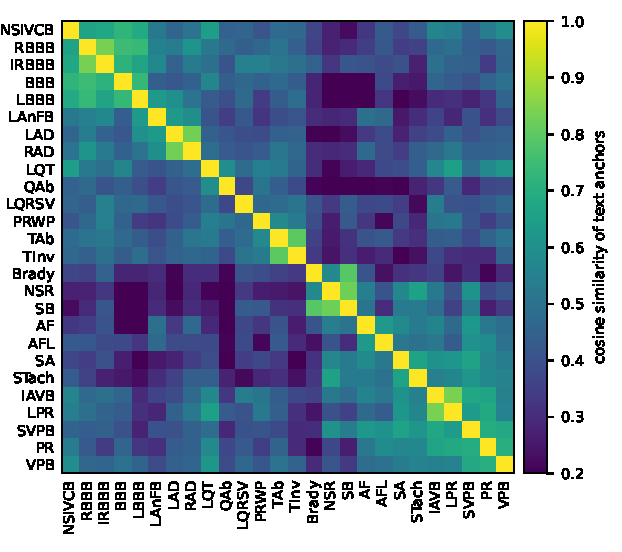
\includegraphics[width=0.78\textwidth]{figures/fig_text_similarity.pdf}
\caption{Cosine similarity between the frozen text anchors $\mathbf{t}_c$ (BioLORD-2023, full descriptions) of the 26 PhysioNet/CinC 2021 scored diagnoses (25 of them are in our vocabulary; poor R-wave progression does not occur in the four databases), ordered by average-linkage hierarchical clustering. Abbreviations follow Supplementary Table~S1.}\label{fig:textsim}
\end{figure}

\subsection{Annotation-aware objective}\label{sec:objective}
\paragraph{Masked asymmetric loss.}
With logit $\ell$, probability $p=\sigma(\ell)$ and target $y$, we use the asymmetric loss~\cite{ridnik_asl}
\begin{equation}
\phi(\ell,y) = -y\log p-(1-y)\,p_m^{\gamma}\log(1-p_m),\qquad p_m=\max(p-m,0),
\label{eq:asl}
\end{equation}
with $\gamma=2$ and $m=0.05$, which down-weights easy negatives in the strongly imbalanced multi-label setting. Only observed entries contribute, and each record is normalized by its number of observed entries so that records from sources with small vocabularies are not down-weighted. For a head with logits $\boldsymbol{\ell}$,
\begin{equation}
\Lann(\boldsymbol{\ell}) = \frac{1}{B}\sum_{i=1}^{B}\frac{\sum_{c} a_{ic}\,\phi\big(\ell_c(\mathbf{x}_i),y_{ic}\big)}{\max\big(1,\sum_c a_{ic}\big)} .
\label{eq:lann}
\end{equation}
Both heads are trained with the same targets and the same mask,
\begin{equation}
\mathcal{L}=\Lann(\boldsymbol{\ell}^{\mathrm{lin}})+\lambda_{\mathrm{txt}}\,\Lann(\boldsymbol{\ell}^{\mathrm{txt}}),\qquad \lambda_{\mathrm{txt}}=1,
\label{eq:total}
\end{equation}
so that the text head is a second, open-vocabulary reading of the same supervision and the encoder receives gradients from both. No term in $\mathcal{L}$ involves an unobserved entry.

\paragraph{Implication completion.}
A set $\mathcal{R}$ of seven clinical implication rules of the form child$\,\rightarrow\,$implied finding (Table~\ref{tab:rules}), for example right bundle branch block $\rightarrow$ bundle branch block, sinus bradycardia $\rightarrow$ bradycardia and first-degree atrioventricular block $\rightarrow$ prolonged PR interval, is applied to the training targets before the loss is computed:
\begin{equation}
y_{ic'}\leftarrow\max(y_{ic'},y_{ic}),\qquad a_{ic'}\leftarrow\max(a_{ic'},y_{ic'})\qquad\text{for }(c\rightarrow c')\in\mathcal{R},
\label{eq:rules}
\end{equation}
so that a completed positive is treated as observed even when the source never codes the implied finding. The rules encode clinical implication, not the SNOMED-CT \emph{is-a} hierarchy. Completion adds positives but never negatives, so a diagnosis that is supervised only through completion has positive-only supervision. Evaluation always uses the original, uncompleted labels.

\subsection{Training, weight averaging, inference and complexity}\label{sec:train}
Algorithm~\ref{alg:step} summarizes one training step. Models are trained for 30 epochs with AdamW (learning rate $10^{-3}$, weight decay $10^{-2}$), a one-cycle learning-rate schedule with 10\% warm-up, batch size $B=256$ and mixed precision; the last incomplete batch of each epoch is dropped. All methods share the random 10\,s crops, per-record amplitude scaling by a factor drawn from $U(0.8,1.2)$, additive Gaussian noise with standard deviation $0.02$\,mV, and lead dropout in which each lead is zeroed independently with probability $0.1$.

\paragraph{Weight averaging.}
After every optimization step $t$ an exponential moving average of the parameters is updated~\cite{tarvainen2017},
\begin{equation}
\bar\theta\leftarrow\mu_t\bar\theta+(1-\mu_t)\theta,\qquad \mu_t=\min\!\Big(\mu,\ \frac{1+t}{10+t}\Big),\quad \mu=0.999,
\label{eq:ema}
\end{equation}
where the warm-up of $\mu_t$ ensures that $\bar\theta$ does not retain a sizeable share of the random initialization during the first epochs (with a constant $\mu=0.999$, about a fifth of the initial weights would still be present after the first 1{,}600 steps). Batch-normalization statistics are copied rather than averaged. The averaged weights $\bar\theta$ are the ones that are validated after each epoch, selected, thresholded and tested. Weight averaging is applied identically to every baseline in our comparison, because in preliminary runs it improved all methods, and leaving it out of the baselines would have confounded the comparison (Appendix~\ref{secA2}).

\paragraph{Model selection and thresholds.}
After every epoch the averaged model is evaluated on a validation split drawn from the training sources, and the checkpoint with the highest macro AUROC over the diagnoses evaluable in that split is retained. Validation AUROC and the F1 thresholds are computed only over observed entries of the original, uncompleted labels: for each diagnosis, over the validation records whose source annotates it, so that model selection does not reward treating unknown entries as negatives. Per-diagnosis decision thresholds are chosen on the same split to maximize F1 over a grid from 0.02 to 0.98 in steps of 0.02. The target database is never used for model selection or threshold tuning. At inference each record is scored by averaging the probabilities of Eq.~\eqref{eq:fusion} over all 10\,s windows at a 5\,s stride that fall inside its valid part.

\paragraph{Complexity.}
The text head adds, per record, self-attention over $C$ queries and cross-attention from $C$ queries to $T$ tokens, i.e.\ $\mathcal{O}(C^2D+CTD)$ operations, which for $C=43$ and $T=32$ is small relative to the convolutional encoder. The hybrid model has 4.62\,M trainable parameters: 3.35\,M in the encoder, 11\,k in the linear head and 1.27\,M in the text-anchored head; the baselines have 3.36\,M (encoder and linear head). The frozen text encoder is used only once, offline, to compute the anchors, so the deployed model needs no language model. A training run on the leave-one-database-out protocol takes a median of 12 minutes on a single cloud GPU, against 10 minutes for the masked baseline.

\begin{algorithm}[!htbp]
\caption{One training step of the proposed method.}\label{alg:step}
\begin{algorithmic}[1]
\Require mini-batch $\{(\mathbf{x}_i,\mathbf{y}_i,\mathbf{a}_i)\}_{i=1}^{B}$ with completed targets (Eq.~\eqref{eq:rules}); anchors $\{\mathbf{t}_c\}$; parameters $\theta$; averaged parameters $\bar\theta$; step $t$
\State $\mathbf{x}^{\mathrm{c}}_i \gets \textsc{RandomCrop}_{10\,\mathrm{s}}(\mathbf{x}_i)$ for all $i$ \Comment{inside the valid part of each record}
\State $\mathbf{x}^{\mathrm{a}}_i \gets \textsc{Augment}(\mathbf{x}^{\mathrm{c}}_i)$ \Comment{amplitude scaling, noise, lead dropout}
\State $\mathbf{H}_i \gets f_\theta(\mathbf{x}^{\mathrm{a}}_i)$ \Comment{shared tokens}
\State $\boldsymbol{\ell}^{\mathrm{lin}}_i \gets \mathbf{W}_{\mathrm{lin}}\bar{\mathbf{h}}_i+\mathbf{b}_{\mathrm{lin}}$;\quad $\boldsymbol{\ell}^{\mathrm{txt}}_i \gets \textsc{TextHead}(\mathbf{H}_i,\{\mathbf{t}_c\})$ \Comment{Eqs.~\eqref{eq:linear}--\eqref{eq:logit}}
\State $\mathcal{L}\gets\Lann(\boldsymbol{\ell}^{\mathrm{lin}})+\lambda_{\mathrm{txt}}\Lann(\boldsymbol{\ell}^{\mathrm{txt}})$ \Comment{Eqs.~\eqref{eq:lann}, \eqref{eq:total}; observed entries only}
\State $\theta\gets\textsc{AdamW}(\theta,\nabla_\theta\mathcal{L})$; advance the one-cycle schedule
\State $\mu_t\gets\min(\mu,(1+t)/(10+t))$;\quad $\bar\theta\gets\mu_t\bar\theta+(1-\mu_t)\theta$ \Comment{Eq.~\eqref{eq:ema}}
\end{algorithmic}
\end{algorithm}
